\documentclass[12pt,fleqn]{beamer}


\xdefinecolor{lavendar}{rgb}{0.8,0.6,1}
\xdefinecolor{olive}{cmyk}{0.64,0,0.95,0.4}
%\xdefinecolor{olive}{cmyk}{1,0,0,0}
\xdefinecolor{mag}{cmyk}{0.1,1,0,0.2}
\xdefinecolor{lblue}{rgb}{0,0,1.5}
\xdefinecolor{lred}{rgb}{1,0,0}
\xdefinecolor{mine}{cmyk}{1,0,0.2,0}
\xdefinecolor{bluel}{cmyk}{0.1,0,0.9,0.4}

\usepackage{amsmath,amssymb,dsfont,mathrsfs}
\usepackage{tikz,pgflibraryplotmarks}
\usepackage{multimedia}
\usepackage{wasysym}
\usepackage{rotating}
\usepackage{algorithm,algorithmic}
\usepackage{graphicx} % more modern
\usepackage{subfigure}
\usepackage{booktabs}

\usepackage{pgfplots}
\usepackage{verbatim}

\usepackage{setspace}
\newlength\iwidth
\newlength\iheight

\newcommand\makebeamertitle{\frame{\maketitle}}%
\graphicspath{{./images/}}
\setbeamertemplate{navigation symbols}{}
\addtobeamertemplate{navigation symbols}{}{%
    \usebeamerfont{footline}%
    \usebeamercolor[fg]{footline}%
	\insertshorttitle
    \;--
    \insertframenumber
}

\newcommand{\sectionstart}{
	\only<beamer>{
 	\begin{frame}% (fold)
 		\begin{centering}\Huge \insertsection \par\end{centering}
 	\end{frame}% frame the_application (end)
	}
 }


% make bibliography entries smaller
\usepackage{natbib}
\setbeamertemplate{bibliography item}{[\theenumiv]}
\renewcommand\bibfont{\scriptsize}
\setbeamertemplate{frametitle continuation}[from second]
\newcommand{\tcr}{\textcolor{red}}
\newcommand{\tcrd}{\textcolor{red}}
\newcommand{\tcb}{\textcolor{bluel}}
\newcommand{\tcm}{\textcolor{mag}}
\newcommand{\tcg}{\textcolor{olive}}

\newcommand{\R}{\mathbb{R}}
\newcommand{\C}{\mathbb{C}}

% bold lower-case for vectors
\newcommand{\bfa}{{\bf a}}
\newcommand{\bfb}{{\bf b}}
\newcommand{\bfc}{{\bf c}}
\newcommand{\bfs}{{\bf s}}
\newcommand{\bfm}{{\bf m}}
\newcommand{\bfd}{{\bf d}}
\newcommand{\bfe}{{\bf e}}
\newcommand{\bfu}{{\bf u}}
\newcommand{\bfy}{{\bf y}}
\newcommand{\bfx}{{\bf x}}
\newcommand{\bfh}{{\bf h}}
\newcommand{\bfw}{{\bf w}}
\newcommand{\bfv}{{\bf v}}
\newcommand{\bfr}{{\bf r}}
\newcommand{\bfz}{{\bf z}}
\newcommand{\bfp}{{\bf p}}


% bold upper-case for linear operators
\newcommand{\bfA}{{\bf A}}
\newcommand{\bfB}{{\bf B}}
\newcommand{\bfZ}{{\bf Z}}
\newcommand{\bfM}{{\bf M}}
\newcommand{\bfC}{{\bf C}}
\newcommand{\bfD}{{\bf D}}
\newcommand{\bfQ}{{\bf Q}}
\newcommand{\bfJ}{{\bf J}}
\newcommand{\bfG}{{\bf G}}
\newcommand{\bfI}{{\bf I}}
\newcommand{\bfP}{{\bf P}}
\newcommand{\bfK}{{\bf K}}
\newcommand{\bfY}{{\bf Y}}
\newcommand{\bfW}{{\bf W}}
\newcommand{\bfR}{{\bf R}}
\newcommand{\bfL}{{\bf L}}
\newcommand{\bfF}{{\bf F}}
\newcommand{\bfT}{{\bf T}}
\newcommand{\bfS}{{\bf S}}
\newcommand{\bfX}{{\bf X}}
\newcommand{\bfU}{{\bf U}}
\newcommand{\bfV}{{\bf V}}
\newcommand{\bfH}{{\bf H}}


\newcommand{\calF}{\mathcal{F}}



\newcommand{\hf}{{\frac 12}}
\newcommand{\bftheta}{{\boldsymbol \theta}}
\newcommand{\bfxi}{{\boldsymbol \xi}}

\newcommand{\bfLambda}{{\boldsymbol \Lambda}}
\newcommand{\bfSigma}{{\boldsymbol \Sigma}}
\newcommand{\bfepsilon}{{\boldsymbol \epsilon}}

\newcommand{\E}{\vec E}
\newcommand{\B}{\vec B}

\newcommand{\vu}{  {\vec {\bf u}}}

\newcommand{\grad}{  {\vec {\bf \nabla}}}

\newcommand{\lfrownie}{\textcolor{red}{\large{\frownie}}}
\newcommand{\lsmiley}{\textcolor{green}{\large{\smiley}}}

\newcommand{\curl}{\ensuremath{\nabla\times\,}}
\renewcommand{\div}{\nabla\cdot\,}
\newcommand{\divh}{\nabla_h\cdot\,}
\renewcommand{\grad}{\ensuremath{\nabla}}

\DeclareMathOperator*{\argmin}{arg\,min}
\date{}

\title{Application of CNN - Image segmentation}
\subtitle{Numerical Methods for Deep Learning}

\begin{document}

\makebeamertitle


\begin{frame}[fragile]\frametitle{Image Segmentation}

The problem:
Given an image $\bfY:R^2 \rightarrow R$
compute probability maps for $n_c$ classes, i.e., for $j=1,\ldots,n_c$
$$\bfP_j:R^2 \rightarrow [0,1], \quad \sum_{j=1}^{n_c} \bfP_j = 1$$

\begin{tabular}{cc}
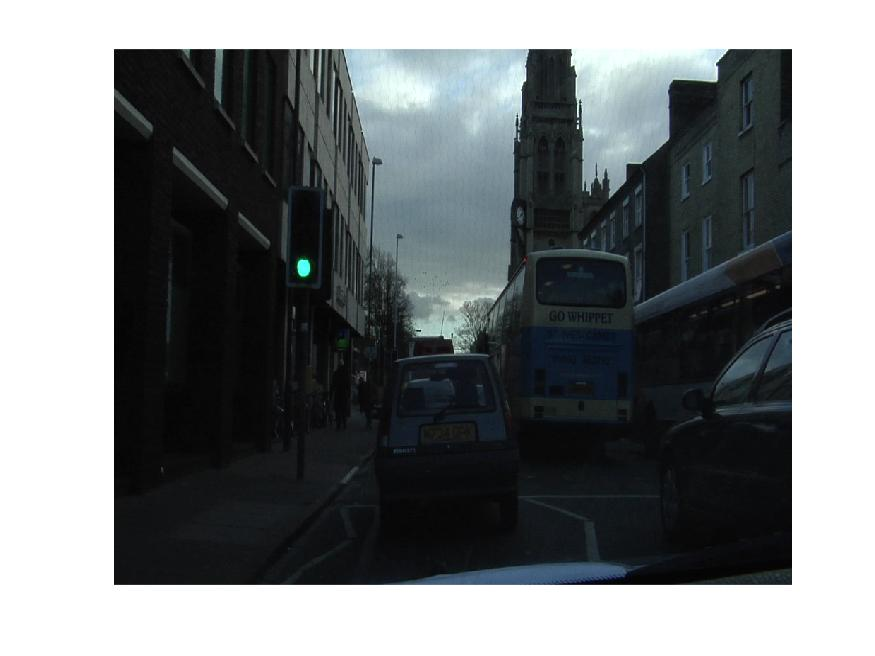
\includegraphics[width=5cm]{camvidPic} &
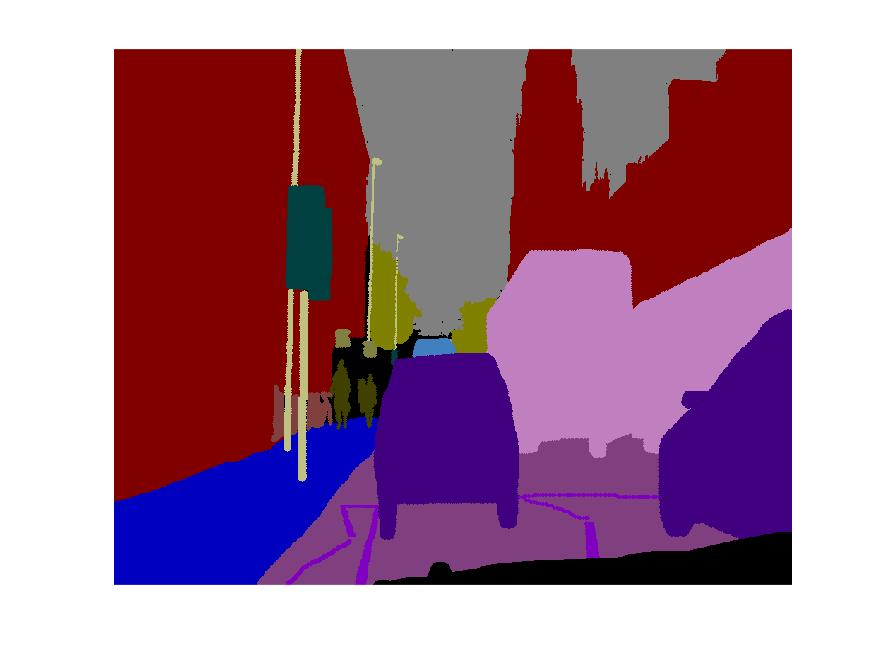
\includegraphics[width=5cm]{camvidClass}
\end{tabular} 


$\bfP_j$ is the probability of a pixel to belong to class $j$ 

\end{frame}

\begin{frame}[fragile]\frametitle{Setup of Image Segmentation Problem}


\begin{itemize}
\item Use a neural network: original image  $\rightarrow n_c$ ``images''
\item Output image represents class probabilities for each pixel
\item Loss: average cross entropy for \textbf{each pixel}
\item Optimize over network parameters
\end{itemize}

\bigskip

Simple example: a single layer and linear classification

\end{frame}


\begin{frame}[fragile]\frametitle{Image Segmentation with Single-Layer NN}

Let $\bfY_0 \in \R^{n\times n_f}$ with $n_f = n_1 \cdot n_2 \cdot 3$ ($n_1\times n_2$ RGB data)

$$ \bfY_1 = \sigma(\bfY_0 \bfK(\theta) + \bfB \bfb). $$

Use 2D convolutions for $\bfK(\theta)$ and assume $k$ output channels, i.e.,
$$ \bfK = \begin{pmatrix}
\bfK_{2D}(\theta_{11}) & \bfK_{2D}(\theta_{12}) & \cdots & \bfK_{2D}(\theta_{1k}) \\
\bfK_{2D}(\theta_{21}) & \bfK_{2D}(\theta_{22}) & \cdots & \bfK_{2D}(\theta_{2k}) \\
\bfK_{2D}(\theta_{31}) & \bfK_{2D}(\theta_{32}) & \cdots & \bfK_{2D}(\theta_{3k}) \\
\end{pmatrix}. $$

Then we have to classify each pixel in $\bfY_1$ using $\bfW \in \R^{k \times n_c}$. This gives the problem
$$
\min_{\bfW,\bfK,\bfb} E({\rm reshape}(\bfY_1) \bfW , \bfP), \qquad \bfY_1 =\sigma(\bfY_0 \bfK(\theta) + \bfB \bfb)
$$
Here ${\rm reshape}(\bfY_1) \in \R^{(n\cdot n_1 \cdot n_2) \times k}$ and $E$ is our cross entropy

\end{frame}

\begin{frame}[allowframebreaks]
	\frametitle{References}
\bibliographystyle{abbrv}
\bibliography{NumDNN}

\end{frame}


\end{document}
















